\section{User Interface}
\label{section:ui}

%\begin{figure*}[th!]
%  \centering
%  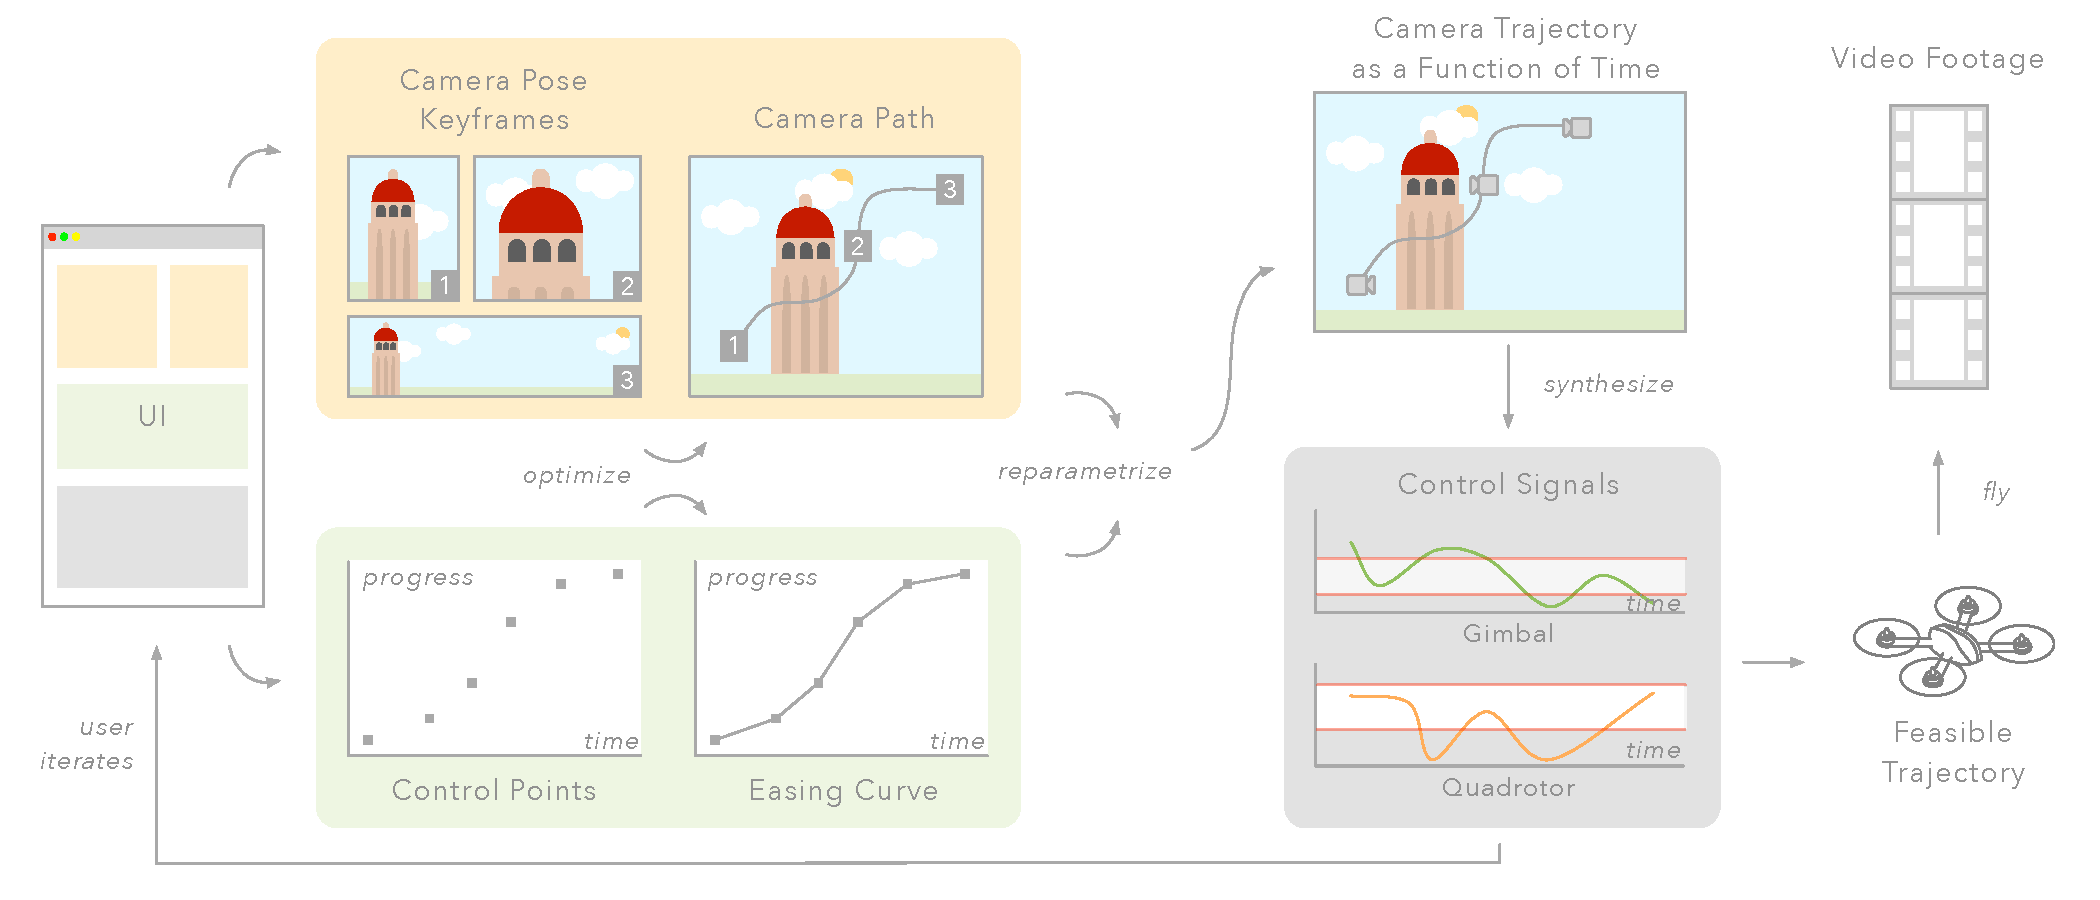
\includegraphics[width=5.5in]{images/system_overview}
%  \caption{
%Overview of the major technical components of our system.
%We begin with two user-specified inputs: (1) camera pose keyframes in a virtual environment (e.g., \textsc{Google Earth}); and (2) a sequence of easing curve control points.
%From these inputs, we compute a smooth camera path and a smooth easing curve.
%We optimize the smoothness of the camera path and easing curve in a way that obeys the physical equations of motion for quadrotors.
%We re-paramterize the camera path, according to the easing curve, to produce a camera trajectory as a function of time.
%We synthesize the control signals required for a quadrotor and gimbal to follow the camera trajectory.
%We plot these control signals in our user interface, providing the user with visual feedback about the physical feasibility of the resulting trajectory.
%The user can edit the resulting trajectory by editing camera pose keyframes and easing curve control points.
%Once the user is satisfied with the trajectory, we command a quadrotor camera to execute the trajectory fully autonomously, capturing real video footage.
%  }
%  \label{figure:overview}
%\end{figure*}

We reify the design principles described in Section \ref{section:design} into an interactive tool for planning and capturing quadrotor camera shots (Figure \ref{fig:teaser}).
In our tool, the user specifies camera pose keyframes at specific times in a virtual environment.
Our tool synthesizes a camera trajectory that obeys the physical equations of motion for quadrotors, and interpolates between the user-specified keyframes.

In our tool, a camera pose \emph{keyframe} consists of a \emph{look-at} position, and a \emph{look-from} position.
Our tool interpolates these vectors separately to synthesize a camera pose \emph{trajectory}.
For simplicity, we always set the camera's \emph{up} vector equal to the world-frame \emph{up} vector.
If artistic control of the camera's \emph{up} vector is desired, our keyframe representation could be straightforwardly modified to include an \emph{up} vector. 

\paragraph{Editing the Visual Content and Timing of Shots}

Our tool provides a 3D view of a virtual scene using \textsc{Google Earth} (Figure \ref{fig:teaser}a).
The user can set keyframes in this view by moving the virtual camera using a trackball interface.
This interface enables the user to design shots visually.
Our tool also provides a 2D map view of the scene using \textsc{Google Maps} (Figure \ref{fig:teaser}b).
The user can set keyframes in this view by dragging look-from and look-at markers around the 2D map.

The user can add, edit, and delete keyframes using the 3D scene view and the 2D map view.
These views are linked: edits in one view instantly update the other view.
Whenever a keyframe is added, edited, or deleted, our tool synthesizes a new camera trajectory in real-time.
Our tool draws the camera trajectory on the 2D map view as a curve, and in the 3D scene view as a rollercoaster-style track, to support spatial awareness.

The user can also change the total duration of her shot, and navigate through time using a scrubber interface (Figure \ref{fig:teaser}c). To set a keyframe at a specific time, the user scrubs to that moment in time and edits the camera pose, as described above.
When the user clicks the \emph{Play} button or moves the scrubber, our tool instantly plays back a preview of the shot.
This functionality, when combined with our strategy for reasoning about the physical feasibility of camera trajectories, allows the user to accurately preview her shot, and supports rapid iteration.

The user can edit distinct easing curves for look-at and look-from position trajectories (Figure \ref{fig:teaser}d).
The user can add, edit, and delete control points on these easing curves.
%For example, in Figure \ref{fig:teaser}d, the second control point on the look-from easing curve was added to slow the camera down.
Editing these easing curves enables the user to precisely control the timing control of her shot.

%The user can also calibrate the virtual camera's field of view to match her real-world camera (Figure \ref{fig:teaser}e).
%The user can adjust the lighting of the virtual environment by adjusting the sun position (Figure \ref{fig:teaser}a).
%These features improve the accuracy of the  virtual preview in our tool.

\paragraph{Fixing Physically Infeasible Shots}

Our tool synthesizes camera trajectories that are guaranteed to obey the physical equations of motion for quadrotors. However, the user can specify shots in our tool that exceed the physical limits of her quadrotor hardware.
For example, the user might specify two keyframes so close together in time, but so far apart in space, that her quadrotor cannot fly fast enough to capture the shot.
Our tool provides the user with visual feedback about the physical feasibility of her trajectory, notifying the user if her intended trajectory violates the physical limits of her  hardware.

Every time the user edits her shot, our tool re-calculates dynamic and kinematic quantities of interest along the camera trajectory in real-time (e.g., gimbal joint angles, velocities, and thrust forces).
Our tool plots these quantities on a set of \emph{feasibility plots} (Figure \ref{fig:teaser}f).
In each plot, our tool shows the physical limits of the quantity with two horizontal red lines.
If any dynamic or kinematic quantity exceeds these physical limits, our tool highlights the corresponding feasibility plot.
Our tool also highlights any infeasible regions directly in the 3D scene view (Figure \ref{fig:teaser}a), the 2D map view (Figure \ref{fig:teaser}b), and on the easing curves (Figure \ref{fig:teaser}d).
In each of these views, our tool colors each point along the trajectory according to the magnitude of the feasibility violations that occur at that point.
Based on this visual feedback, the user can adapt her shot to the physical limits of her hardware.

\paragraph{Capturing Real Video Footage}

At any time during the design process, the user can save her shot.
Once the user is pleased with her shot, she can take a laptop running our tool, and her quadrotor, to the approximate real-world starting location of her shot.
The user can initiate an automatic capture session by clicking the \emph{Start Capture} button (Figure \ref{fig:teaser}g).
Once the user clicks this button, our tool commands a quadrotor camera to execute the user-specified shot fully autonomously, capturing real video footage.
